%!TEX root = ../dokumentation.tex

% Deckblatt für Bachelorarbeit
% Cover page for bachelor thesis

\begin{titlepage}
	\begin{longtable}{p{8.2cm} p{5.4cm}}
		{\raisebox{\ht\strutbox-\totalheight}{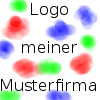
\includegraphics{images/firmenlogo.png}}} &
		{\raisebox{\ht\strutbox-\totalheight}{\includegraphics[height=2.5cm]{images/dhbw.png}}}
	\end{longtable}
	\enlargethispage{20mm}
	\begin{center}
		\vspace*{12mm}	{\LARGE\textbf \thesistitle }\\
		\vspace*{12mm}	{\large\textbf \thesistype}\\
		\vspace*{12mm}	\langcoverclosinginstructions\\
		\vspace*{3mm}		{\textbf \degree}\\
		\vspace*{12mm}	\langarticlecourseofstudies{} \langcourseofstudies{} \courseofstudies\\
		\vspace*{3mm}		\langatthedh{} \dhbwcity\\
		\vspace*{12mm}	\langby\\
		\vspace*{3mm}		{\large\textbf \thesisauthor}\\
		\vspace*{12mm}	\submissiondate\\
	\end{center}
	\vfill
	\begin{spacing}{1.2}
		\begin{tabbing}
			mmmmmmmmmmmmmmmmmmmmmmmmmm             \= \kill
			\textbf{\langcstimeofproject}       \>  \timeperiod\\
			\textbf{\langcsstudentid, \langcscourse}  \>  \studentid, \course\\
			\textbf{\langcscompany}                  \>  \company, \copmanylocation\\
			\textbf{\langcssupervisor}               \>  \supervisor\\
			\textbf{\langcsreviewer}              \>  \reviewer
		\end{tabbing}
	\end{spacing}
\end{titlepage}